
\chapter{Week1}

\section{Tuesday}\index{Tuesday_lecture}
\subsection{Introduction and Examples}
$u(x,y)$ a smooth function\\
$u_x=\frac{\partial u}{\partial x}$\\
$u_y=\frac{\partial u}{\partial y}$\\
$u_{xx}=\frac{\partial ^2u}{\partial x\partial x}$\\
$u_{xy}=\frac{\partial ^2u}{\partial y\partial x}$\\
In this course, as $u$ is smooth, we don't fuss about difference between $u_{xy}$ and $u_{yx}$.\\
\begin{definition}
A PDE is a relation for $F(x,y,u,u_x,y_y,u_{xy},\dots)=0$
linear equation.  If $F$ is linear in $u$, $u_x$, $u_y$, $u_{xx}$, $\cdots$ (Not necessarily in $x$, $y$)
\end{definition}

\begin{example}
Laplace equation: $u_{xx} + u_{xy} = 0$\\
$( x^2 + y^2 ) u_{xx} + e^{xy} u_{yy} = 0$\\
In the second case, it is still linear as it is a linear equation for $u_{xx}$ and $u_{yy}$. 
\end{example}
Other examples\\
Cauchy-Riemann.\\

$\begin{cases}
u_x - v_y = 0 \\
u_y + v_x = 0
\end{cases}$ 1st order system\\
$\begin{cases}u_{xx}-v_{yx}=0\\u_{yy}+v_{yx}\end{cases}\rightarrow u_{xx}+y_{yy}=0$ harmonic function ($2^{\text{st}}$ order).\\
Order: highest order that partial derivatives are taken.\\
Notation for laplace operator:
\[\Delta u=u_{xx}+u_{yy},~ \Delta u=u_{xx},~ \Delta u=u_{x_1x_1}+\cdots +u_{x_nx_n}\]
\begin{example}
Wave equation. $u_{tt}=c^2\Delta u$, $c>0$ wave speed a constant, $t$: time.\\
$n=1$ $u_tt=c^2u_{xx}$: vibration of a string\\
$n=2$ $u_{tt}=c^2(u_{xx}+u_{yy})$: water wave\\
$n=3$ $u_{tt}=c^2(u_{x_1x_1}+u_{x_2x_2}+u_{x_3x_3})$: sound wave\\
n: space dimension\\
n=1 A string, flexible, elastic, homogeneous with density $\rho$
\begin{figure}[H]
\centering
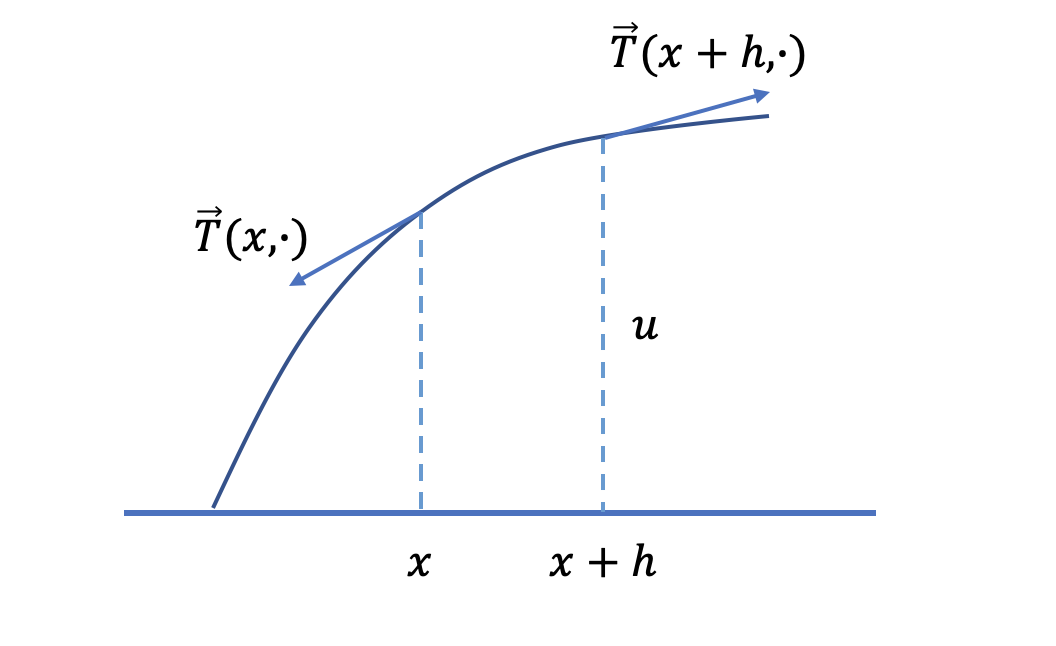
\includegraphics[width=10cm]{week1_tuesday1}
\end{figure}
\begin{figure}[H]
\centering
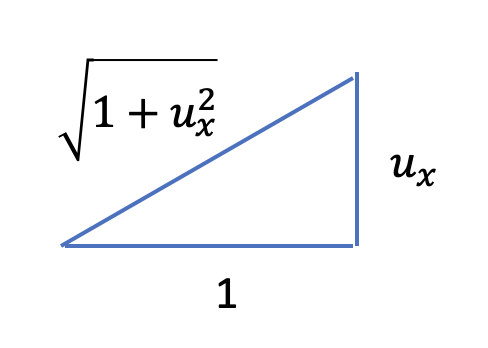
\includegraphics[width=6cm]{week1_tuesday2}
\end{figure}
When we magnefy part of the string and let $h$ to be small enough. The horizontal parts of  forces of $\vec{T}(x,\cdot)$ and $\vec{T}(x+h,\cdot)$ are equal to each other. Vertical forces is equal to $am$ according to Newton's second law. Therefore, we have the following.
\[\left\{\begin{gathered}\frac{|T|(x+h,\cdot)}{\sqrt{1+u_x^2(x+h,\cdot)}}=\frac{|T|(x,\cdot)}{\sqrt{1+u_x^2(x,\cdot)}}\\\frac{|T|u_x}{\sqrt{1+u_x^2}}(x+h,\cdot)-\frac{|T|u_x}{\sqrt{1+u_x^2}}(x,\cdot)=h\rho u_{tt}\end{gathered}\right.
\]
When $h$ is small enough,
\[\frac{1}{\sqrt{1+u_x^2}}=(1+u_x^2)^{-\frac{1}{2}}=1-\frac{1}{2}u_x^2+\cdots\approx1
\]
\[|T|(x+h,\cdot)=|T|(x,\cdot)
\]
\[\rho u_{tt}=|T|\cdot[u_x(x+h,\cdot)-u_x(x,\cdot)]\frac{1}{h}\rightarrow |T|u_{xx}
\]
\[u_{tt}=\frac{|T|}{\rho}u_{xx},~ c=\sqrt{\frac{|T|}{\rho}}
\]

\end{example}
\begin{example}[Heat equation]
$u_t=\Delta u$, u: temprature\\
$\begin{aligned}H(t)&=\text{total amount of heat in } \Omega\subset\mathbb{R}^3\\
&=\underset{\Omega}{\int\int\int}c\rho u \diff x\diff y\diff z
\end{aligned}$
\[\underset{\partial\Omega}{\int\int}\kappa\vartriangle u \nu\diff s=\frac{\diff H}{\diff t}=\underset{\Omega}{\int\int\int}c\rho u \diff x\diff y\diff z
\]
$\kappa$ is heat conduction constant. $\nu$ is unit outward normal.\\
\[\vec{w}=\vartriangle u=(u_x,u_y,u_z)
\]
\[\text{dir} \vec{w}=u_{xx}+u_{yy}+u_{zz}=\Delta u
\]
By divergent theorem:
\[\underset{\Omega}{\int\int\int}c\rho u_t=\underset{\Omega}{\int\int\int}\kappa\Delta u
\]
As this is the case for all $\Omega$ we can tell $c\rho u_t=\kappa\Delta u$
\[u_t=\frac{\kappa}{c\rho}{\Delta u}
\]
\end{example}
\begin{theorem}[Divergent theorem]
$\vec{w}=(w_1,w_2,w_3)$: vector field\\
\[\underset{\Omega}{\int\int\int}\text{dir}\vec{w}\diff x\diff y\diff z=\underset{\partial\Omega}{\int\int}\vec{w}\nu\diff s
\]
where $\text{dir}\vec{w}=\frac{\partial w_1}{\partial x}+\frac{\partial w_2}{\partial y}+\frac{\partial w_3}{\partial z}$




\end{theorem}







